\documentclass[11pt]{article}
\usepackage[utf8]{inputenc}
\usepackage[spanish]{babel}
\usepackage{graphicx}         % Para incluir imágenes
\usepackage{amsmath}          % Para notación matemática
\usepackage{amssymb}          % Para símbolos matemáticos como \mathbb
\usepackage[margin=3cm]{geometry}  % Márgenes
\usepackage[font=normalsize,labelfont=small]{caption}  % Estilo de captions
\usepackage{hyperref}         % Para links clickeables

% EXTENSIÓN MÁXIMA: 10 HOJAS SIN EXCEPCIÓN.
\begin{document}

\begin{titlepage}
    \centering
    \vspace*{2cm}
    
\includegraphics[scale=0.8]{Logo-Udesa.jpg}\par
    \vspace{30pt}

    {\LARGE \textbf{I302 - Aprendizaje Automático\\ y Aprendizaje Profundo}\par}
    \vspace{1cm}

    {\LARGE \textbf{Trabajo Práctico 2: \\Clasificación y Ensemble Learning}\par}
    \vspace{2cm}
    
    {\LARGE {Eliana Ostrovsky}\par}
    \vspace{2cm}
    
    {\Large \today\par}
    \vspace{1cm}
    \Large{Ingeniería en Inteligencia Artificial}
\end{titlepage}

% EJERCICIO 1
\section{Diagnóstico de Cáncer de Mama}
% RESUMEN
\begin{abstract}
    En este trabajo se quiso modelar el diagnóstico de cáncer de mama a partir de características celulares. Para llevarlo a cabo, se desarrolló un modelo de regresión logística binaria con regularización L2 y se evaluaron distintas técnicas de rebalanceo. Se probó utilizando datos balanceados y desbalanceados. El modelo performó correctamente, alcanzando un F-score de 0.93 en datos balanceados y de 0.85 con cost re-weighting. Las métricas mostraron un buen equilibrio entre precisión y recall en ambos casos.
\end{abstract}

% INTRODUCCION
\subsection{Introducción}
El objetivo del presente trabajo fue modelar el diagnóstico de cáncer de mama a partir de características celulares extraídas de imágenes histopatológicas. La entrada del algoritmo consiste en un conjunto de variables numéricas que describen propiedades morfológicas y moleculares de las células, como el tamaño y forma del núcleo, la tasa de mitosis, la densidad nuclear y la presencia de ciertas mutaciones genéticas.

Se desarrolló un modelo de regresión logística binaria con regularización L2, cuyo objetivo es predecir si un tumor es benigno o maligno. Este modelo fue entrenado y evaluado sobre distintos conjuntos de datos, tanto balanceados como desbalanceados. En este último caso, se aplicaron diversas estrategias de rebalanceo con el fin de mejorar la detección de la clase minoritaria, que representa los casos clínicamente más críticos.
%     Explicar el problema. Proporcionar el contexto necesario y explicar cuáles son las entradas y salidas del algoritmo. Por ejemplo: “La entrada del algoritmo es (imagen, amplitud de señal, edad del paciente, mediciones de lluvia, video en escala de grises, etc.). Luego, se utilizó un/a (red neuronal, regresión lineal, árbol de decisión, etc.) para obtener una predicción de (edad, precio de acciones, tipo de cáncer, género musical, etc.)”.}

% METODOS
% \subsection{Métodos}
% \textit{Describir los algoritmos que se implementaron y utilizaron. Asegurarse de incluir la notación matemática relevante. Si el espacio lo permite, se podrá dar una breve descripción ($\approx$ 1 párrafo) de cómo funciona.}

% \textit{Describir el conjunto de datos: ¿Qué proporción de entrenamiento/validación/prueba se utilizó? ¿Se realizó algún preprocesamiento? ¿Qué tipo de normalización o aumento de datos se utilizó?}

% \textit{Detallar los hiperparámetros elegidos y cómo se seleccionaron. ¿Realizaron validación cruzada? Si es así, ¿cuántos folds utilizaron?}

% \textit{Incluir métricas de rendimiento utilizadas.}

\subsection{Métodos}

Para abordar el problema de clasificación binaria, se implementó desde cero un modelo de \textit{regresión logística} con regularización L2. El objetivo de este modelo es estimar la probabilidad de que una observación pertenezca a la clase positiva (tumor maligno), dada una entrada $\mathbf{x} \in \mathbb{R}^d$ con $d$ características.

La probabilidad estimada se modela como:

\[
\hat{y} = \sigma(\mathbf{w}^\top \mathbf{x} + b) = \frac{1}{1 + e^{-(\mathbf{w}^\top \mathbf{x} + b)}}
\]

donde $\sigma(\cdot)$ es la función sigmoide, $\mathbf{w}$ es el vector de pesos y $b$ el sesgo. Para entrenar el modelo, se minimizó la función de pérdida logarítmica con penalización L2:

\[
\mathcal{L}(\mathbf{w}, b) = -\frac{1}{N} \sum_{i=1}^N \left[ y^{(i)} \log \hat{y}^{(i)} + (1 - y^{(i)}) \log (1 - \hat{y}^{(i)}) \right] + \frac{\lambda}{2} \|\mathbf{w}\|^2
\]

donde $y^{(i)}$ es la etiqueta verdadera, $\hat{y}^{(i)}$ la probabilidad predicha y $\lambda$ el hiperparámetro de regularización. La optimización se realizó mediante descenso por gradiente con tasa de aprendizaje constante.

\vspace{0.3cm}
\noindent \textbf{Conjunto de datos y preprocesamiento.} \\
Se utilizaron tres conjuntos de datos: uno balanceado para entrenamiento y prueba, y otro desbalanceado para evaluar distintas estrategias de rebalanceo. En todos los casos, los datos se dividieron en un 80\% para entrenamiento y 20\% para validación, manteniendo la proporción de clases mediante muestreo estratificado para los conjuntos desbalanceados. 

El preprocesamiento incluyó varias etapas: primero, se aplicaron límites para restringir los valores de variables específicas a rangos biológicamente plausibles. Luego, para el tratamiento de outliers, se implementó un enfoque de agrupamiento mediante K-means con dos clústeres para cada característica numérica, aplicando el método del rango intercuartílico (IQR) dentro de cada clúster. Para el manejo de valores faltantes, se utilizó un método de imputación basado en k-vecinos más cercanos (k-NN), donde para cada valor faltante se identificaron los k=5 vecinos más cercanos y se imputó la media de sus valores. Finalmente, se aplicó normalización estándar (z-score) a todas las características numéricas.

Las características categóricas como 'CellType' fueron transformadas mediante codificación one-hot, resultando en variables binarias como 'Epthlial' y 'Mesnchymal', mientras que 'GeneticMutation' fue convertida directamente a una variable binaria.

\vspace{0.3cm}
\noindent \textbf{Selección de hiperparámetros.} \\
El valor del hiperparámetro de regularización $\lambda$ se seleccionó utilizando búsqueda en grilla sobre el conjunto de validación, evaluando múltiples valores logarítmicamente espaciados entre $10^{-1}$ y $10^4$. Se seleccionó el modelo con mejor F1-score en el conjunto de validación, resultando en un valor óptimo de $\lambda = 0.1$.

\vspace{0.3cm}
\noindent \textbf{Estrategias de rebalanceo.} \\
Sobre el conjunto desbalanceado, se aplicaron cinco enfoques para tratar el desequilibrio de clases:
\begin{itemize}
    \item \textit{Sin rebalanceo}: entrenamiento directo sobre datos desbalanceados.
    \item \textit{Undersampling}: eliminación aleatoria de muestras de la clase mayoritaria hasta igualar ambas clases.
    \item \textit{Oversampling por duplicación}: replicación aleatoria de muestras de la clase minoritaria hasta igualar ambas clases.
    \item \textit{SMOTE} (Synthetic Minority Over-sampling TEchnique): generación de muestras sintéticas para la clase minoritaria mediante interpolación lineal entre muestras existentes y sus k vecinos más cercanos.
    \item \textit{Cost re-weighting}: ponderación en la función de pérdida de acuerdo a la proporción inversa de cada clase, dando mayor peso a la clase minoritaria.
\end{itemize}

\vspace{0.3cm}
\noindent \textbf{Métricas de evaluación.} \\
Para evaluar el desempeño del modelo se utilizaron múltiples métricas: \textit{accuracy}, \textit{precision}, \textit{recall}, \textit{F-score}, matriz de confusión, curva ROC y curva Precision-Recall (PR), junto con el área bajo cada curva (AUC-ROC y AUC-PR). El F-score fue utilizado como criterio principal para la selección de hiperparámetros y la comparación entre estrategias de rebalanceo.

\subsection{Resultados}

El modelo de regresión logística con regularización L2 mostró un rendimiento sólido tanto en los datos balanceados como en los desbalanceados. En esta sección se analizan los resultados de ambos escenarios.

\subsubsection{Datos Balanceados}

Utilizando el conjunto balanceado, el modelo de regresión logística alcanzó un F-score de 0.93 en el conjunto de validación, con una precisión y recall igualmente altos (0.97 y 0.90 respectivamente para la clase negativa, 0.90 y 0.97 para la positiva). La matriz de confusión (Figura 1) muestra un equilibrio adecuado entre falsos positivos y falsos negativos, lo que es crucial en el contexto del diagnóstico médico.

\begin{figure}[h]
    \centering
    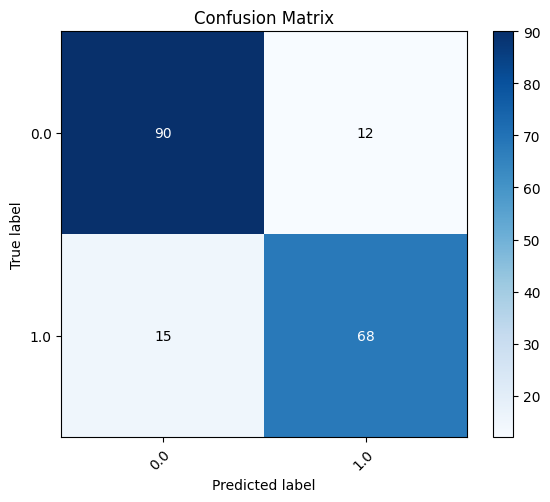
\includegraphics[width=0.8\textwidth]{figuras/confusion_matrix_balanced.png}
    \caption{Matriz de confusión para el modelo entrenado con datos balanceados. Se observa un buen equilibrio entre falsos positivos (9) y falsos negativos (5).}
    \label{fig:confusion_matrix_balanced}
\end{figure}

Al evaluar el modelo sobre el conjunto de prueba balanceado, el rendimiento se mantuvo relativamente estable con un F-score de 0.85, mostrando la robustez del modelo ante datos no vistos. La ligera disminución en el rendimiento es esperada y sugiere que el modelo no sufre de sobreajuste severo.

\subsubsection{Datos Desbalanceados y Estrategias de Rebalanceo}

Para el conjunto desbalanceado, donde aproximadamente el 25\% de las muestras correspondían a tumores malignos, se implementaron diversas estrategias de rebalanceo. La Tabla 1 resume las métricas obtenidas para cada enfoque.

\begin{table}[h]
\centering
\caption{Comparación de métricas para las diferentes estrategias de rebalanceo}
\label{tab:rebalancing_metrics}
\begin{tabular}{lcccccc}
\hline
\textbf{Modelo} & \textbf{Accuracy} & \textbf{Precision} & \textbf{Recall} & \textbf{F-Score} & \textbf{AUC-ROC} & \textbf{AUC-PR} \\
\hline
Sin rebalanceo & 0.9156 & 0.7857 & 0.9167 & 0.8462 & 0.9650 & 0.8754 \\
Undersampling & 0.9156 & 0.7500 & 1.0000 & 0.8571 & 0.9664 & 0.8807 \\
Oversampling duplicate & 0.9241 & 0.7692 & 1.0000 & 0.8696 & 0.9651 & 0.8741 \\
Oversampling SMOTE & 0.9241 & 0.7692 & 1.0000 & 0.8696 & 0.9647 & 0.8778 \\
Cost re-weighting & 0.9114 & 0.7407 & 1.0000 & 0.8511 & 0.9639 & 0.8735 \\
\hline
\end{tabular}
\end{table}

Las curvas ROC y Precision-Recall (Figura 2) permiten una comparación visual del rendimiento de los distintos enfoques. Todas las curvas ROC muestran valores de AUC superiores a 0.96, indicando una excelente capacidad discriminativa del modelo independientemente de la estrategia de rebalanceo empleada.

\begin{figure}[h]
    \centering
    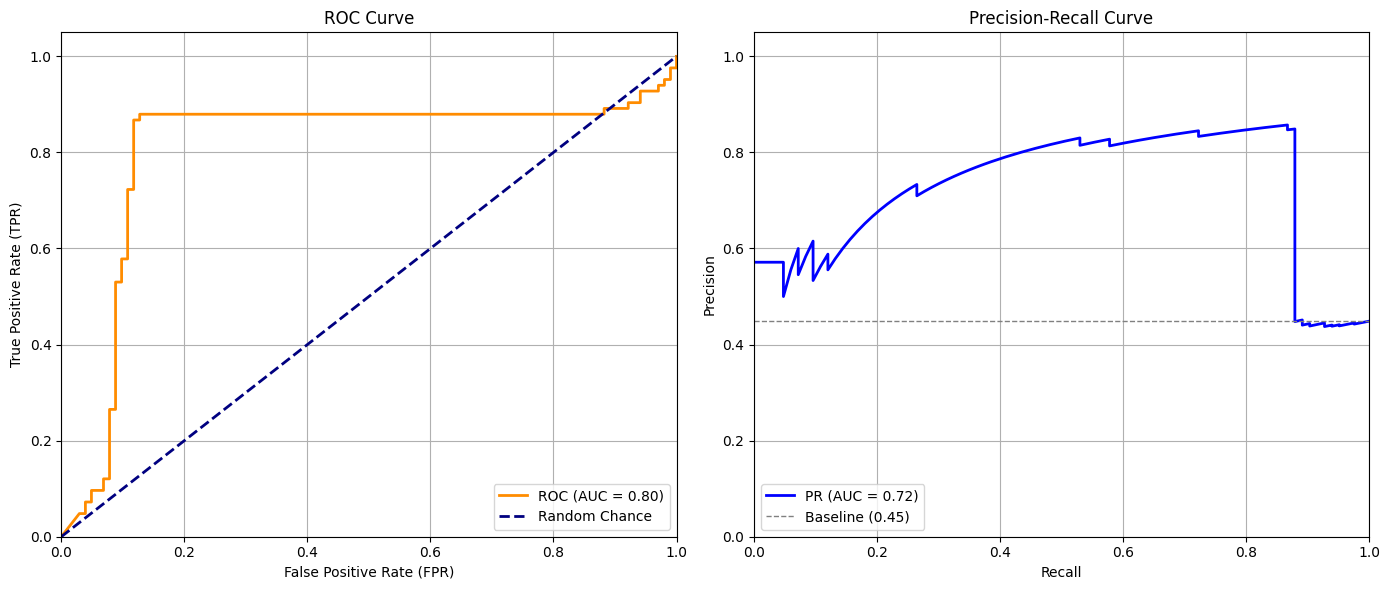
\includegraphics[width=\textwidth]{figuras/roc_pr_curves.png}
    \caption{Curvas ROC (izquierda) y Precision-Recall (derecha) para las diferentes estrategias de rebalanceo. Todas las estrategias logran un rendimiento similar en términos de AUC.}
    \label{fig:roc_pr_curves}
\end{figure}

Entre las estrategias evaluadas, los métodos de oversampling (tanto por duplicación como SMOTE) obtuvieron el F-score más alto (0.8696), con un recall perfecto (1.0) para la clase positiva (tumores malignos) y una precisión aceptable (0.7692). El undersampling mostró un comportamiento similar pero con una precisión ligeramente menor. La estrategia de cost re-weighting, aunque presentó el F-score más bajo entre los métodos de rebalanceo, aún superó al modelo sin rebalanceo en términos de recall.

Para la evaluación final en el conjunto de prueba desbalanceado, se seleccionó el modelo con oversampling por duplicación, obteniendo un F-score de 0.80 para la clase positiva y un recall de 0.88, confirmando su capacidad para identificar correctamente la mayoría de los casos malignos, lo cual es prioritario en el contexto clínico donde es preferible reducir los falsos negativos a costa de aumentar ligeramente los falsos positivos.

\subsubsection{Discusión de Resultados}

Los resultados muestran que las técnicas de rebalanceo mejoran significativamente la capacidad del modelo para detectar tumores malignos en conjuntos desbalanceados, donde predominan los casos benignos. El incremento en el recall para la clase positiva es particularmente relevante, ya que en aplicaciones médicas como el diagnóstico de cáncer, el costo de no detectar un caso positivo (falso negativo) es considerablemente mayor que el de clasificar erróneamente un caso negativo como positivo (falso positivo).

Las técnicas de oversampling y undersampling obtuvieron resultados comparables, aunque el oversampling tendió a mantener una mejor precisión. Esto sugiere que la pérdida de información debido a la eliminación de muestras en undersampling puede afectar negativamente la capacidad del modelo para discriminar correctamente entre casos difíciles.

Es notable que todas las estrategias de rebalanceo lograron un recall perfecto (1.0) en el conjunto de validación, lo que indica que estos métodos son efectivos para sensibilizar al modelo hacia la clase minoritaria. Sin embargo, este incremento en recall viene a costa de una disminución en la precisión, evidenciando el conocido compromiso precision-recall.

La estrategia de cost re-weighting, aunque conceptualmente diferente al no modificar la distribución de los datos sino la función de pérdida, mostró un comportamiento similar a las técnicas de resampling, confirmando que existen múltiples enfoques viables para abordar el problema del desbalanceo de clases.

% EJERCICIO 2
\section{Predicción de Rendimiento de Jugadores de Basketball}
% RESUMEN
\begin{abstract}
En este trabajo se modeló el rendimiento de jugadores de basketball mediante clasificación multiclase. Para llevarlo a cabo, se desarrollaron e implementaron tres algoritmos desde cero: Análisis Discriminante Lineal (LDA), Regresión Logística Multiclase y Random Forest. Se probaron utilizando métricas como accuracy, precision, recall y F-score. El modelo de Random Forest performó notablemente mejor, alcanzando 95.2\% de exactitud y 0.99 de AUC-ROC en el conjunto de prueba, superando a los modelos de LDA y Regresión Logística que mostraron rendimientos similares entre sí con exactitudes de 90.5\% y 91.7\% respectivamente.
\end{abstract}

% INTRODUCCION
\subsection{Introducción}
Este trabajo aborda el problema de predicción del rendimiento de jugadores de basketball utilizando técnicas de aprendizaje automático para clasificación multiclase. La entrada del algoritmo consiste en un conjunto de variables numéricas que describen métricas de rendimiento individual de los jugadores, como minutos jugados (mp), posesiones en la temporada (poss), rating ofensivo y defensivo (raptor\_total) e impacto en el ritmo del juego (pace\_impact).

El objetivo es predecir la clase de WAR (Wins Above Replacement) a la que pertenece cada jugador, que representa el impacto del jugador en términos de partidos ganados por encima de lo que aportaría un jugador suplente promedio. Esta métrica se categorizó en tres clases: WAR Negativo (clase 1), WAR Nulo (clase 2) y WAR Positivo (clase 3).

Para abordar este problema de clasificación multiclase, se implementaron y compararon tres modelos diferentes: Análisis Discriminante Lineal (LDA), Regresión Logística Multiclase con regularización L2, y Random Forest con optimización de hiperparámetros, evaluando su capacidad para distinguir correctamente entre las tres categorías de impacto de los jugadores.

% METODOS
\subsection{Métodos}

Para este problema de clasificación multiclase, se implementaron tres modelos diferentes, cada uno con una aproximación distinta al problema:

\vspace{0.3cm}
\noindent \textbf{Análisis Discriminante Lineal (LDA)} \\
El modelo LDA asume que los datos de cada clase siguen una distribución gaussiana multivariada con matriz de covarianza compartida entre clases. Bajo esta premisa, la probabilidad de que una observación $\mathbf{x}$ pertenezca a la clase $k$ viene dada por la regla de Bayes:

\[
P(y = k | \mathbf{x}) \propto P(\mathbf{x} | y = k) \cdot P(y = k) = \mathcal{N}(\mathbf{x} | \boldsymbol{\mu}_k, \mathbf{\Sigma}) \cdot \pi_k
\]

donde $\boldsymbol{\mu}_k$ es el vector de medias para la clase $k$, $\mathbf{\Sigma}$ es la matriz de covarianza compartida y $\pi_k$ es la probabilidad a priori de la clase $k$. La clasificación se realiza asignando la observación a la clase con mayor probabilidad posterior.

\vspace{0.3cm}
\noindent \textbf{Regresión Logística Multiclase} \\
El modelo de regresión logística multiclase estima la probabilidad de que una observación pertenezca a cada una de las clases mediante la función softmax:

\[
P(y = k | \mathbf{x}) = \frac{e^{\mathbf{w}_k^T \mathbf{x} + b_k}}{\sum_{j=1}^K e^{\mathbf{w}_j^T \mathbf{x} + b_j}}
\]

donde $\mathbf{w}_k$ es el vector de pesos para la clase $k$, $b_k$ es el sesgo correspondiente, y $K$ es el número total de clases. Se utilizó regularización L2 para prevenir el sobreajuste, modificando la función de pérdida logarítmica de la siguiente manera:

\[
\mathcal{L}(\mathbf{W}, \mathbf{b}) = -\frac{1}{N} \sum_{i=1}^N \sum_{k=1}^K y_{ik} \log(p_{ik}) + \frac{\lambda}{2} \sum_{k=1}^K \|\mathbf{w}_k\|^2
\]

donde $y_{ik}$ es 1 si el ejemplo $i$ pertenece a la clase $k$ y 0 en caso contrario, $p_{ik}$ es la probabilidad predicha, y $\lambda$ es el parámetro de regularización.

\vspace{0.3cm}
\noindent \textbf{Random Forest} \\
El modelo de Random Forest es un conjunto de árboles de decisión que utiliza técnicas de bagging (bootstrap aggregating) y selección aleatoria de características para mejorar la generalización. Cada árbol se entrena sobre una muestra bootstrap de los datos originales y, en cada nodo, considera solo un subconjunto aleatorio de las características disponibles para realizar la división. La predicción final se obtiene mediante votación mayoritaria entre todos los árboles.

\vspace{0.3cm}
\noindent \textbf{Conjunto de datos y preprocesamiento} \\
El conjunto de datos WAR\_class\_dev.csv contiene 6,782 observaciones con 5 variables predictoras y la variable objetivo war\_class. Se comprobó que no existieran valores faltantes ni datos duplicados. El conjunto presentaba un ligero desbalanceo entre clases: 30\% para clase 1 (WAR Negativo), 37\% para clase 2 (WAR Nulo) y 33\% para clase 3 (WAR Positivo).

Los datos se dividieron en 80\% para entrenamiento y 20\% para validación. Antes del entrenamiento, se aplicó normalización estándar (z-score) a todas las características numéricas, guardando las medias y desviaciones estándar del conjunto de entrenamiento para aplicar la misma transformación al conjunto de validación y, posteriormente, al de prueba.

\vspace{0.3cm}
\noindent \textbf{Selección de hiperparámetros} \\
Para la regresión logística multiclase, se utilizó una tasa de aprendizaje de 0.1, 1000 iteraciones y un parámetro de regularización $\lambda = 0.1$.

Para el Random Forest, se realizó una búsqueda exhaustiva de hiperparámetros mediante validación cruzada con 5 folds, evaluando 7 configuraciones diferentes en las que se variaron: número de árboles (100-150), profundidad máxima (5-10 o sin límite), mínimo número de muestras para división (2-5) y proporción de características a considerar en cada división (todas o 70\%). El F1-score ponderado fue la métrica utilizada para seleccionar la mejor configuración, resultando en: 150 árboles, profundidad máxima de 8, mínimo de 5 muestras para dividir un nodo y uso del 70\% de las características en cada división.

\vspace{0.3cm}
\noindent \textbf{Métricas de evaluación} \\
Los modelos se evaluaron utilizando múltiples métricas:
\begin{itemize}
    \item Exactitud (Accuracy): proporción de predicciones correctas.
    \item Precisión (Precision): proporción de predicciones positivas correctas.
    \item Recall: proporción de muestras positivas reales identificadas correctamente.
    \item F1-Score: media armónica entre precisión y recall.
    \item Matriz de confusión: visualización de predicciones correctas e incorrectas.
    \item Curvas ROC y Precision-Recall, con sus respectivas áreas bajo la curva (AUC-ROC y AUC-PR).
\end{itemize}

% RESULTADOS
\subsection{Resultados}

Los tres modelos implementados fueron evaluados en el conjunto de validación y posteriormente en el conjunto de prueba independiente. La Tabla 1 muestra las métricas principales obtenidas en el conjunto de prueba.

\begin{table}[h]
\centering
\caption{Comparación de rendimiento de los modelos en el conjunto de prueba}
\label{tab:model_comparison}
\begin{tabular}{lcccccc}
\hline
\textbf{Modelo} & \textbf{Accuracy} & \textbf{Precision} & \textbf{Recall} & \textbf{F1-Score} & \textbf{AUC-ROC} & \textbf{AUC-PR} \\
\hline
LDA & 0.9051 & 0.9153 & 0.9051 & 0.9101 & 0.9691 & 0.9266 \\
Regresión Logística & 0.9169 & 0.9197 & 0.9169 & 0.9183 & 0.9686 & 0.9215 \\
Random Forest & \textbf{0.9522} & \textbf{0.9540} & \textbf{0.9522} & \textbf{0.9531} & \textbf{0.9928} & \textbf{0.9877} \\
\hline
\end{tabular}
\end{table}

El modelo Random Forest superó claramente a los otros dos enfoques en todas las métricas evaluadas, alcanzando una exactitud del 95.22\% y un AUC-ROC de 0.993. Las matrices de confusión (Figura 1) revelan patrones interesantes en los errores de clasificación de cada modelo.

\begin{figure}[h]
    \centering
    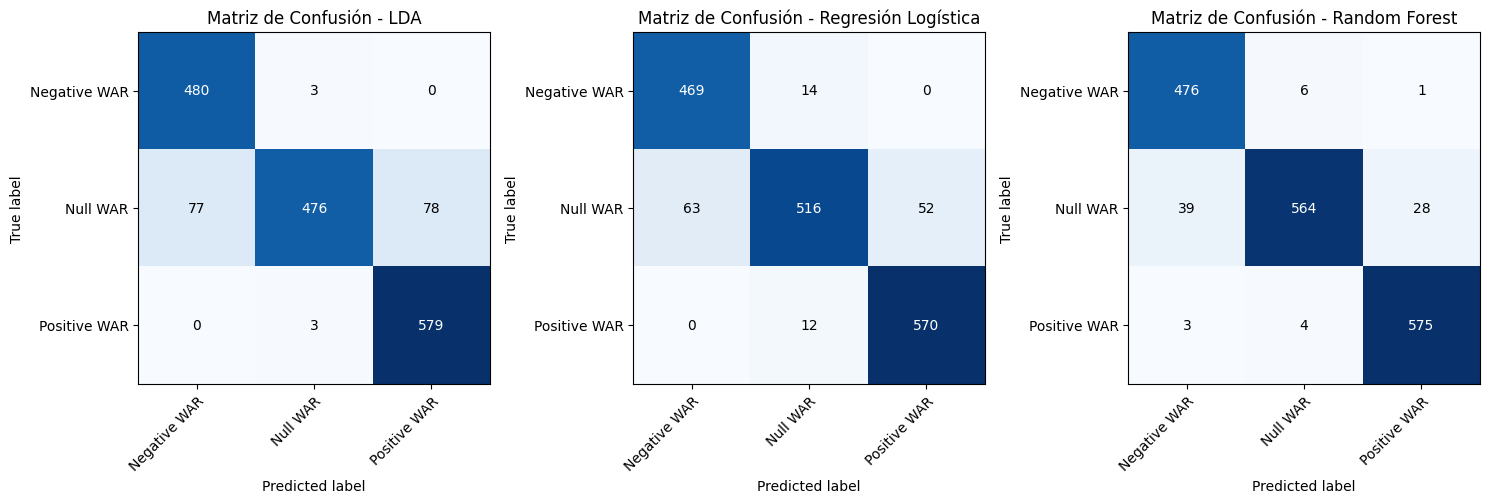
\includegraphics[width=\textwidth]{figuras/confusion_matrices.png}
    \caption{Matrices de confusión para los tres modelos evaluados en el conjunto de prueba. De izquierda a derecha: LDA, Regresión Logística y Random Forest.}
    \label{fig:confusion_matrices}
\end{figure}

El análisis de las matrices de confusión muestra que el modelo LDA tuvo dificultades particulares para clasificar la clase 2 (WAR Nulo), con 77 ejemplos incorrectamente clasificados como clase 1 y 78 como clase 3. La regresión logística mejoró ligeramente la clasificación de la clase 2, pero seguía confundiendo algunos casos con la clase 1. El Random Forest logró una clasificación mucho más precisa de todas las clases, aunque mantuvo un patrón similar de confusión entre clases adyacentes.

La comparación entre las métricas obtenidas en validación y prueba muestra una buena consistencia para los tres modelos, lo que indica que las estimaciones de error mediante validación cruzada fueron confiables. El Random Forest mostró incluso una ligera mejora en el conjunto de prueba respecto a validación (95.22\% vs 91.75\% en exactitud), posiblemente debido a que este modelo pudo aprovecharse de todo el conjunto de desarrollo para su entrenamiento final.

Es interesante notar que todas las clases muestran AUC-ROC superior a 0.97 en el caso del Random Forest, indicando una excelente capacidad de discriminación. El modelo parece captar eficientemente las relaciones entre las variables de entrada y el rendimiento de los jugadores, incluso para los casos fronterizos entre clases adyacentes.

La superioridad del Random Forest probablemente se debe a su capacidad para capturar relaciones no lineales entre las variables y el manejo implícito de interacciones entre características. Esto es particularmente valioso en este contexto, donde el rendimiento de un jugador de baloncesto puede depender de combinaciones complejas de sus estadísticas individuales. Además, el proceso de optimización de hiperparámetros mediante validación cruzada permitió encontrar una configuración que balancea adecuadamente la complejidad del modelo y su capacidad de generalización.

Por otro lado, tanto LDA como la regresión logística, al ser modelos lineales, tienen limitaciones inherentes para capturar patrones complejos en los datos. A pesar de esto, ambos modelos lograron un rendimiento respetable, con exactitudes superiores al 90\%, lo que sugiere que existe una estructura lineal significativa en los datos que estos modelos pudieron aprovechar.

En un entorno de producción, el modelo Random Forest sería la elección más recomendable debido a su superior rendimiento predictivo en todas las métricas. Sin embargo, si la interpretabilidad fuera un factor crítico, la regresión logística podría ser preferible, ya que sus coeficientes proporcionan información directa sobre la influencia de cada variable en la clasificación.


\end{document}




